% Stage 4 report, short version: framed like the Stage 2 and Stage 3 reports (same models, names and
% numbers); the only new part is the ltp tool. Compile from this folder: pdflatex stage4_short.tex (twice).
\documentclass[11pt,a4paper]{article}
\usepackage[margin=2.2cm]{geometry}
\usepackage[T1]{fontenc}
\usepackage{lmodern}
\usepackage{amsmath}
\usepackage{graphicx}
\usepackage{booktabs}
\usepackage{array}
\usepackage{enumitem}
\usepackage{xcolor}
\usepackage{caption}
\usepackage{float}
\usepackage[section]{placeins}
\usepackage[hidelinks]{hyperref}
\graphicspath{{../experiments/}}
\setlist{itemsep=1pt,topsep=3pt}
\setlength{\parindent}{0pt}
\setlength{\parskip}{4pt}
\captionsetup{font=small,labelfont=bf}
\newcommand{\us}{\,$\mu$s}
\newcommand{\degC}{\,\textdegree C}
\newcommand{\todo}[1]{\textcolor{red}{[TODO: #1]}}
\setcounter{tocdepth}{1}

\begin{document}

\begin{center}
{\LARGE\bfseries Lightweight Temperature Predictor:}\\[4pt]
{\Large\bfseries TapaSense}\\[4pt]
{\large Stage 4: Final Report}\\[8pt]
Ethan Bobby Kurien \quad Kaivalya Mase
\end{center}

\begin{abstract}
TapaSense predicts the temperature of every core of a multi-core chip from the core powers. The
HotSpot simulator computes these temperatures accurately, but one steady-state answer takes about
a quarter of a second, while dynamic thermal management (DTM) needs an answer every millisecond.
A one-time calibration runs HotSpot with 1\,W in one core at a time: 8 runs for the steady-state
model and 24 for the transient one. Prediction then uses only the stored coefficients. Because
HotSpot is linear, the steady-state model (an influence matrix) reproduces HotSpot exactly
(0.00003\,K worst) in 2.6\us\ from under 1\,kB. The transient model (a sum of four exponentials)
is off by 0.09\,K on average and 0.30\,K at worst, in 3.1\us\ per step from 3.7\,kB. Without
calibration, every alternative we tried is 0.8--2.8\,K off on average. Both stages are packaged
as one tool, \texttt{ltp}.
\end{abstract}

\tableofcontents

%=====================================================================
\section{Introduction}
A modern chip has several cores. When they work hard they heat up, and if they get too hot they
slow down, wear out faster or fail. The chip's DTM keeps them under a limit by lowering frequency
and voltage. To decide well it needs to know how hot each core is, and ideally how hot it will be
a few milliseconds from now~\cite{coskun09}. HotSpot~\cite{hotspot} computes chip temperatures
accurately, but far too slowly for this.

\textbf{The assignment.} \emph{Develop a lightweight temperature predictor in two stages.
Calibration (one-time per floorplan): tune the predictor's coefficients for the given floorplan
with heterogeneous cores. Prediction: predict the temperature (steady state or transient) for a
given power input.}


%=====================================================================
\section{Design approach}

\subsection{Two stages}
\textbf{Calibration} runs once per floorplan: HotSpot is run a few times with planned inputs and
the coefficients are stored in a model file. \textbf{Prediction} runs many times: it loads the
model file, takes the power of each core, and returns the temperature of every block, either the
steady value or the temperature over time. It does not run HotSpot.

\subsection{Why a linear model can be exact}
HotSpot models the die and its package (silicon, thermal paste, heat spreader, heat sink) as a
large network of thermal resistances and capacitances. Without temperature-dependent leakage this
network is \emph{linear}: if the power doubles, every temperature rise doubles, and the rises
caused by different cores add up. We confirmed this to $10^{-6}$\,K. It follows that the steady
temperature is
\begin{equation}
  T = T_\text{amb} + G\,P,
  \label{eq:s1}
\end{equation}
where $P$ is the vector of core powers (W), $T_\text{amb}$ the ambient temperature, and $G$ the
\emph{influence matrix}: $G_{ij}$ is the steady temperature rise of block $i$ (K) per watt in
core $j$.

\subsection{Models}
\textbf{S1, influence matrix (steady state).} Column $j$ of $G$ is measured directly by one steady
HotSpot run with 1\,W in core $j$ and 0\,W elsewhere:
$G[:,j] = T_\text{HotSpot}(\text{1\,W in core } j) - T_\text{amb}$. That is $N = 8$ runs and no
fitting. Any power vector is a sum of these unit powers, so by linearity S1 is exact.

\textbf{S1-hot-max (hot spots).} A core's hottest point is several kelvin above its average. Each
calibration run also gives HotSpot's full $64\times64$ map, so every grid cell $q$ has its own row
of coefficients $G^\text{cell}_{qj}$, and the hot spot of core $c$ is
$T_\text{hot}(c) = T_\text{amb} + \max_{q\in c} \sum_j G^\text{cell}_{qj} P_j$. It needs no
extra runs.

\textbf{T3, sum of exponentials (transient).} Because HotSpot is linear, its response to any power
trace is fixed by the response to a 1\,W step in each core. Calibration records these step
responses: $s_{ij}(t)$ is the rise of block $i$ at time $t$ after 1\,W is switched on in core $j$.
T3 writes each one as a sum of $M$ rising curves:
\begin{equation}
  s_{ij}(t) \approx \sum_{m=1}^{M} a_{ijm}\left(1 - e^{-t/\tau_m}\right),
  \qquad \sum_m a_{ijm} = G_{ij}.
  \label{eq:t3}
\end{equation}
The time constants $\tau_m$ are the same for every pair of cores; only the weights $a_{ijm}$
differ. The weights of each pair add up to $G_{ij}$, so T3 ends at exactly S1's value.

\textbf{Baselines.} S0, power blurring~\cite{blurring}: one generic heat-spread kernel, no runs on
the target floorplan. T1: one time constant per core. T2, ARX: fitted to one long recorded HotSpot
trace~\cite{coskun09,singla15}.

\subsection{Evaluation}
\begin{itemize}
  \item \textbf{Reference:} HotSpot grid model with $64\times64$ cells, the given layer stack,
        HotSpot's standard package, ambient 45\degC, time step 1\,ms.
  \item \textbf{Test data is never used for calibration.} Steady: the given nominal and maximum
        power and 300 random power vectors per floorplan. Transient: random traces of 2\,s and
        10\,s from a cold chip.
  \item \textbf{Metrics:} mean and worst absolute error over the cores, and the share of cases
        with the right hottest core; time per prediction (median of 10{,}000 calls); model size
        (stored coefficients $\times$ 8 bytes).
\end{itemize}

%=====================================================================
\section{Data}
\begin{center}
\small
\begin{tabular}{@{}l p{9.6cm} c@{}}
\toprule
Set & Description & Floorplans \\
\midrule
Main set & The 23 given floorplans (4 styles) and HET-A, our own heterogeneous layout; every
           floorplan has 2 big (4$\times$4\,mm) and 6 little (2$\times$2\,mm) cores & 24 \\
Generated & Our generator, 13 per style of the given floorplans & 52 \\
\bottomrule
\end{tabular}
\end{center}
\textbf{Power.} Nominal: big 20\,W, little 8\,W (88\,W per chip). Random test vectors: big
10--20\,W, little 5--10\,W. At nominal power the given floorplans reach 69--77\degC, and a little
core is always the hottest: it has 1.6$\times$ the power density of a big core.

%=====================================================================
\section{Calibration}
Calibrating one floorplan takes 24 HotSpot runs; the steady model alone needs 8 runs (about 4\,s).
A little core heats itself 2.4$\times$ as much per watt as a big core. The step responses contain
time constants from about 1\,ms to 8\,s, so one time constant cannot fit them, and four can
(Figure~\ref{fig:steps}).

\begin{figure}[H]
  \centering
  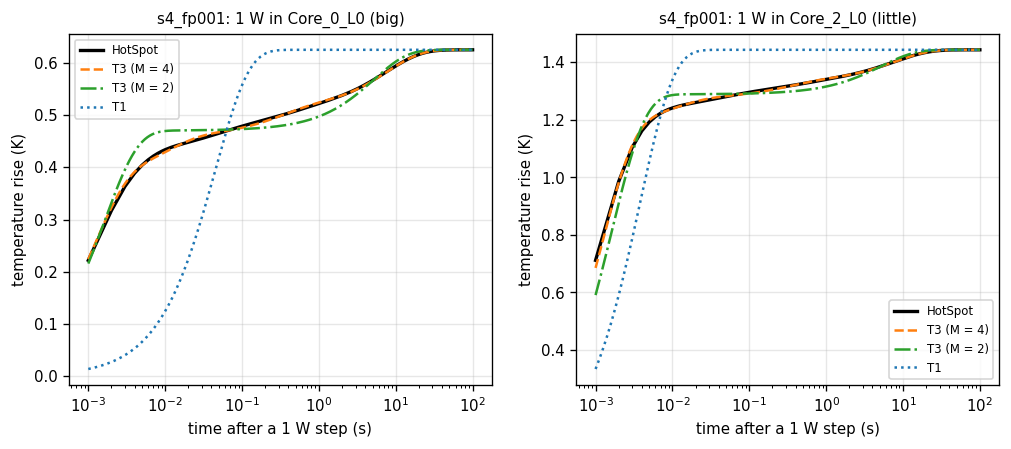
\includegraphics[width=0.75\linewidth]{P1-1_step_calibration/results/step_response_fits_stage3.png}
  \caption{Step responses to 1\,W in a big core (left) and a little core (right), log time axis.
  HotSpot and T3 overlap; T1 has the right final value but the wrong shape.}
  \label{fig:steps}
\end{figure}

\textbf{Is calibration needed? Yes.} We tested calibration-free methods on 6{,}946 unseen HotSpot
runs (the 23 given floorplans):
\begin{center}
\small
\begin{tabular}{@{}l c c c c@{}}
\toprule
Method & Runs on target & Mean error & Worst error & Hottest core right \\
\midrule
\textbf{S1, calibrated} & \textbf{8} & \textbf{0.000007\,K} & \textbf{0.00003\,K} & \textbf{100\,\%} \\
S0 power blurring & 0 & 0.76\,K & 5.2\,K & 71\,\% \\
Borrow $G$, same style (Style 4) & 0 & 1.11\,K & 5.2\,K & 60\,\% \\
Borrow $G$, another style & 0 & 2.79\,K & 12.1\,K & 46\,\% \\
\bottomrule
\end{tabular}
\end{center}
Even on Style~4, where only the core positions differ, borrowing another floorplan's $G$ is
1.1\,K off: die edges, distances between cores and die size make every $G$ unique.

%=====================================================================
\section{Steady-state results}
\begin{center}
\small
\begin{tabular}{@{}l c c c c c@{}}
\toprule
Model (7{,}248 runs, 24 floorplans) & Mean error & Worst error & Time & Size & vs HotSpot \\
\midrule
S0 (no calibration) & 0.77\,K & 5.2\,K & 2.5\us & 928\,B & 94{,}000$\times$ \\
\textbf{S1} & \textbf{0.000006\,K} & \textbf{0.00003\,K} & \textbf{2.6\us} & \textbf{928\,B} & \textbf{91{,}000$\times$} \\
\bottomrule
\end{tabular}
\end{center}
S1 is exact to HotSpot's 6-decimal output and always picks the right hottest core; in 32-bit
numbers it is 464\,B. $G$ grows with the square of the number of cores, but even on a 64-core chip
it is only 32.8\,kB.

\textbf{Hot spots.} The core average underestimates the real peak, so a limit applied to core
averages would let the hot spot run several kelvin hotter. S1-hot-max is exact:
\begin{center}
\small
\begin{tabular}{@{}l c c c c@{}}
\toprule
Model (1{,}380 runs) & Size & Mean error & Worst error & Hottest core right \\
\midrule
Core average (plain S1) & 512\,B & 2.73\,K & 8.96\,K & 50\,\% \\
\textbf{S1-hot-max} & \textbf{115\,kB} & \textbf{0.000007\,K} & \textbf{0.00003\,K} & \textbf{100\,\%} \\
\quad 32-bit & 57\,kB & 0.000007\,K & 0.00003\,K & 100\,\% \\
\bottomrule
\end{tabular}
\end{center}

%=====================================================================
\section{Transient results}
\begin{center}
\small
\begin{tabular}{@{}l c c c c@{}}
\toprule
Model (24 floorplans, 2\,s traces) & Mean error & Worst error & Time per step & Size \\
\midrule
T1 (one time constant per core) & 7.25\,K & 14.6\,K & 1.5\us & 1.0\,kB \\
T2 ARX(2,2) & 0.19\,K & 0.57\,K & 5.4\us & 6.2\,kB \\
\textbf{T3, $M = 4$} & \textbf{0.090\,K} & \textbf{0.30\,K} & \textbf{3.1\us} & \textbf{3.7\,kB} \\
T3, $M = 6$ & 0.0093\,K & 0.13\,K & 3.2\us & 5.6\,kB \\
\bottomrule
\end{tabular}
\end{center}
We chose T3 with $M = 4$: it meets the targets with room to spare, it is exact in steady state,
and it gives the best accuracy per byte, with $M$ as one knob for more accuracy. T1 cannot cover
1\,ms to 8\,s with one time constant, and ARX is about 2$\times$ less accurate and needs a long
recorded trace.

\begin{figure}[H]
  \centering
  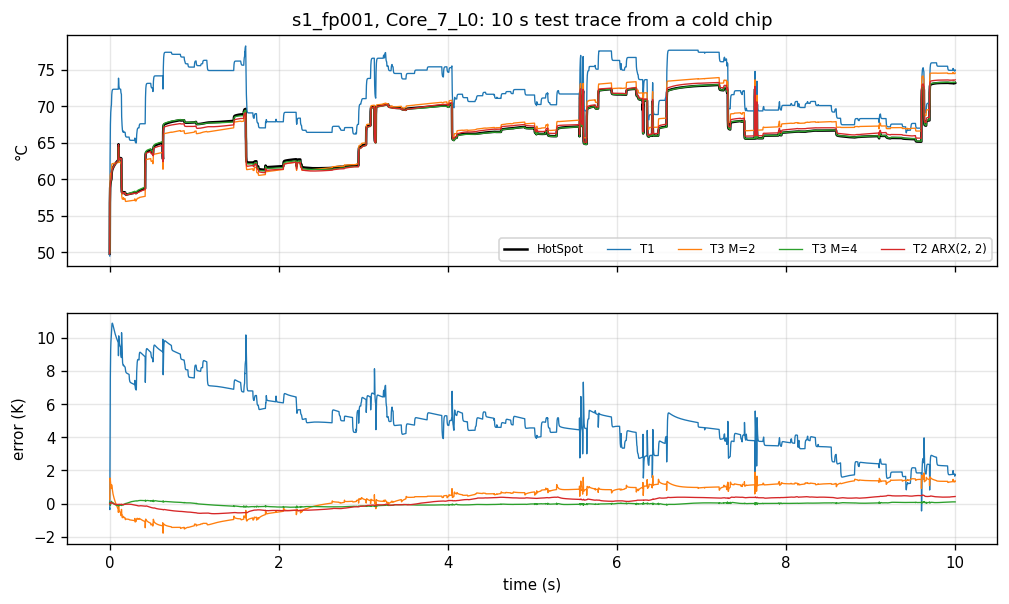
\includegraphics[width=0.65\linewidth]{P3-1_transient_predictor/results/trace_example.png}
  \caption{HotSpot and the models on one 10\,s test trace from a cold chip (top) and their error
  (bottom); T3 sits on top of HotSpot.}
  \label{fig:trace}
\end{figure}

%=====================================================================
\section{Validation on 52 generated floorplans}
The models were developed on the main set. For confirmation we tested them on 52 floorplans they
had never seen, generated in the four given styles with the same cores. The results carry over:
\begin{center}
\small
\begin{tabular}{@{}l c c c c@{}}
\toprule
Set & S1 mean & S1 worst & T3 mean & T3 worst \\
\midrule
52 generated floorplans & $6.5\times10^{-6}$\,K & $3.4\times10^{-5}$\,K & 0.091\,K & 0.34\,K \\
Main set (24 floorplans) & $6\times10^{-6}$\,K & $3\times10^{-5}$\,K & 0.090\,K & 0.30\,K \\
\bottomrule
\end{tabular}
\end{center}

\begin{figure}[H]
  \centering
  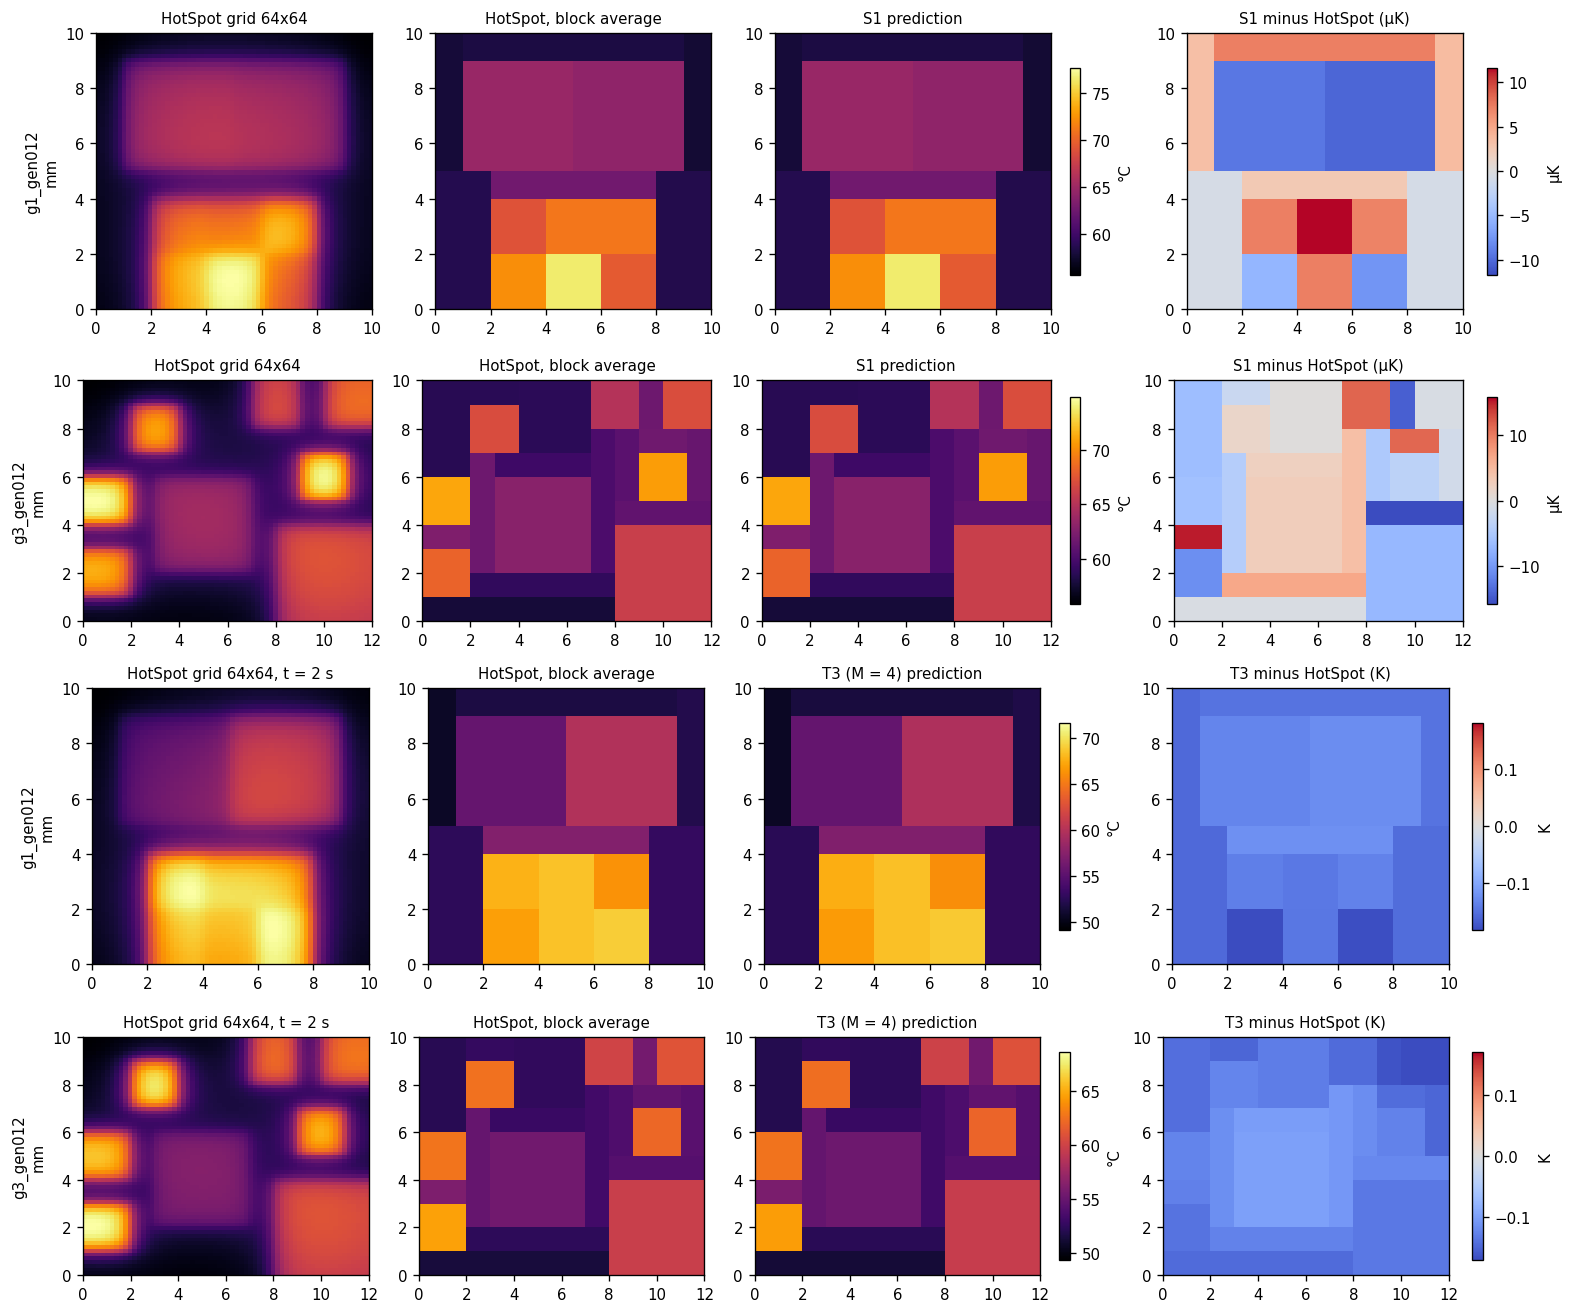
\includegraphics[width=0.75\linewidth]{extended_validation/results/heatmaps_stage4.png}
  \caption{Two generated floorplans (axes in mm). Top two rows: steady state, S1 error in
  micro-kelvin. Bottom two rows: T3 at the end of a 2\,s test trace, error in kelvin. Columns:
  HotSpot's $64\times64$ map, HotSpot's block averages, the prediction, and prediction minus
  HotSpot.}
  \label{fig:maps}
\end{figure}

%=====================================================================
\section{Robustness}
\begin{itemize}
  \item \textbf{Unusual inputs.} Steady power at 3$\times$ the maximum, transients at 2$\times$
        power, bursty power switching every 1--5\,ms, and warm starts all stay within the 1\,K
        target (T3 worst 0.27--0.64\,K).
  \item \textbf{Cooling and ambient.} The coefficients belong to one floorplan \emph{and} one
        package. A new ambient needs no recalibration, only the new $T_\text{amb}$. A new heat
        sink does: the old model is 4.4--8.5\,K off in steady state, and recalibrating restores
        the accuracy.
  \item \textbf{Leakage.} Real chips leak more power when hot, which breaks linearity. Ignoring
        HotSpot's leakage costs 0.08--0.10\,K. Adding the leakage as extra power and repeating
        $T = T_\text{amb} + G\,(P + P_\text{leak}(T))$ removes the error in 3 iterations
        (22--25\us). HotSpot has no transient leakage, so only steady state was tested.
\end{itemize}

%=====================================================================
\section{The \texttt{ltp} tool}
\texttt{ltp} runs both stages. \texttt{calibrate} runs the 24 HotSpot runs (cached, so a second
call reuses them) and writes one model file per floorplan. Every prediction command needs only
that file and NumPy, not HotSpot. \texttt{bench} checks a model file against fresh HotSpot runs.
{\small\begin{verbatim}
python3 -m src.ltp calibrate s4_fp001 -o model.npz      # 24 HotSpot runs, cached
python3 -m src.ltp steady    model.npz --power 20,20,8,8,8,8,8,8
python3 -m src.ltp transient model.npz --ptrace trace.ptrace -o out.ttrace
python3 -m src.ltp bench     model.npz s4_fp001
\end{verbatim}}
On s4\_fp001 the complete model is 8{,}032\,B, a steady prediction takes 2.6\us\ and a transient
step 3.5\us.

%=====================================================================
\section{Scorecard against our targets}
\begin{center}
\small
\begin{tabular}{@{}l l c c c@{}}
\toprule
& Metric & Target & Achieved & Status \\
\midrule
S1 & Mean error per block & $\le 0.1$\,K & 0.000006\,K & met \\
   & Error in the peak & $\le 0.2$\,K & 0.00003\,K & met \\
   & Hottest core right & $\ge 99\,\%$ & 100\,\% & met \\
   & Time per prediction & $\le 20$\us & 2.6\us & met \\
   & Model size & $\le 5$\,kB & 928\,B (464\,B in 32-bit) & met \\
   & Calibration runs & $\le 9$ & 8 (4\,s) & met \\
\midrule
T3 & Mean error over a trace & $\le 0.5$\,K & 0.06--0.09\,K & met \\
   & Error in the peak & $\le 1$\,K & 0.27--0.30\,K & met \\
   & Hottest core right & $\ge 95\,\%$ & 96\,\% (worst floorplan) & met \\
   & Time per step & $\le 50$\us & 3.1\us & met \\
   & Model size & $\le 50$\,kB & 3.7\,kB & met \\
   & Calibration time & $\le 2$\,min wall & $\approx 2.75$\,min & slightly over \\
\bottomrule
\end{tabular}
\end{center}

%=====================================================================
\section{Verification approach}
\begin{enumerate}
  \item Check the reference first: HotSpot's linearity, and block vs grid model.
  \item Keep calibration and test data strictly separate, and test on 52 floorplans generated
        after the models were designed.
  \item Compare every model with a simpler or calibration-free baseline, and stress-test beyond
        nominal conditions.
\end{enumerate}

%=====================================================================
\section{What went as planned, and what deviated}
\textbf{As planned:} the two-stage design; HotSpot as the reference, patched to print 6 decimals so
that errors of $10^{-5}$\,K can be measured; S1 as the steady model; T3 as the transient model;
evaluation on accuracy, time and size; the calibration-is-needed check; robustness studies.

\begin{center}
\small
\begin{tabular}{@{}p{2.6cm} p{4.4cm} p{8cm}@{}}
\toprule
Item & Planned & Done, and why \\
\midrule
HotSpot build & A precision patch & Also faster transients and a memory-leak fix: long traces were
impractical or crashed. \\
Dataset & Our own synthetic floorplans & The 23 given floorplans (plus HET-A) as the main set,
plus 52 generated in the same styles. \\
Hot spots & One hottest cell per core & S1-hot-max over every cell of a core: exact, with no
extra runs. \\
\bottomrule
\end{tabular}
\end{center}

%=====================================================================
\section{Limitations}
\begin{itemize}
  \item All results are against HotSpot, not silicon measurements.
  \item Leakage was tested in steady state only.
  \item A model is tied to its package: a new heat sink needs recalibration.
\end{itemize}

%=====================================================================
\section{Learnings and future scope}
\textbf{Learnings.}
\begin{enumerate}
  \item HotSpot is linear without leakage, so a matrix model can be exact.
  \item Calibration is cheap (8 runs, 4\,s) and needed: position matters, not just core type.
  \item Core averages hide hot spots several kelvin hotter.
  \item Heat moves on time scales from 1\,ms to 8\,s: one time constant fails, four suffice.
  \item Planned step runs beat fitting a recorded trace.
\end{enumerate}
\textbf{Future scope.} Run S1 and T3 inside a controller that throttles or migrates tasks before a
core overheats; leakage in transient prediction, with a simulator that supports it.

%=====================================================================
\section{Presentation feedback}
\begin{center}
\small
\begin{tabular}{@{}l p{6cm} l p{5cm}@{}}
\toprule
\# & Feedback & Incorporated? & Action taken / reason \\
\midrule
1 & \todo{feedback} & \todo{yes/no} & \todo{what was changed, or why not} \\
2 & & & \\
3 & & & \\
\bottomrule
\end{tabular}
\end{center}

%=====================================================================
\section{Submission contents and how to run}
\begin{itemize}
  \item \texttt{reports/}: the reports (PDF and \LaTeX\ source); \texttt{presentations/}: the slides.
  \item \texttt{src/}: implementation (\texttt{sim/} HotSpot tooling, \texttt{ltp/} predictor).
  \item \texttt{experiments/}: one folder per experiment with \texttt{run.py}, README and results.
  \item \texttt{tests/}, \texttt{setup/}, \texttt{configs/}, \texttt{data/}: unit tests, HotSpot
        patches and build script, configurations, floorplans.
  \item \texttt{README\_SETUP.md}: setup and run instructions.
\end{itemize}
Inside WSL, from the repository root:
{\small\begin{verbatim}
bash setup/build_hotspot_ltp.sh                 # one time: build the patched HotSpot
python3 tests/test_models.py                    # unit tests
bash experiments/run.sh <experiment folder>     # run one experiment
\end{verbatim}}

%=====================================================================
\section{LLM assistance disclosure}
LLMs were used to understand HotSpot, for literature review to select appropriate models, to
generate floorplans, to write calibration and testing scripts, and to create this document using
\LaTeX.

\begin{thebibliography}{99}\small
\setlength{\itemsep}{0pt}
\bibitem{hotspot} W.~Huang, S.~Ghosh, S.~Velusamy, K.~Sankaranarayanan, K.~Skadron and
  M.~R. Stan, ``HotSpot: A Compact Thermal Modeling Methodology for Early-Stage VLSI Design,''
  \emph{IEEE TVLSI} 14(5):501--513, 2006.
\bibitem{blurring} A.~Ziabari, J.-H. Park, E.~K. Ardestani, J.~Renau, S.-M. Kang and
  A.~Shakouri, ``Power Blurring: Fast Static and Transient Thermal Analysis Method for Packaged
  Integrated Circuits and Power Devices,'' \emph{IEEE TVLSI} 22(11):2366--2379, 2014.
\bibitem{coskun09} A.~K. Coskun, T.~S. Rosing and K.~C. Gross, ``Utilizing Predictors for
  Efficient Thermal Management in Multiprocessor SoCs,'' \emph{IEEE TCAD} 28(10), 2009.
\bibitem{singla15} G.~Singla, G.~Kaur, A.~K. Unver and U.~Y. Ogras, ``Predictive Dynamic Thermal
  and Power Management for Heterogeneous Mobile Platforms,'' in \emph{Proc. DATE}, 2015.
\end{thebibliography}

\end{document}
